\section{Experimental Evaluation on \ourbenchmark{}}

% \begin{table}[t]
% \begin{center}
% \begin{tabular}{lcc}
% \toprule
% \multicolumn{1}{c}{\bf Model} 
% & \multicolumn{1}{c}{\bf Test set ($N=7k$)} 
% & \multicolumn{1}{c}{\bf Test-unseen-parents ($N=3k$)} \\
% \midrule
% Base (\qwenfourb)        & $6.6$   & $6.698$ \\
% SFT (\qwenfourb)         & $6.456$ & $6.468$ \\
% SFT-think (\qwenfourb)   & $6.674$ & $6.744$ \\
% \gemtwopro{}               & $6.903$ & $7.038$ \\   
% \gemthreepro{}             & $6.866$ & $7.059$ \\ 
% \ourmethod{} (\qwenfourb{} after RL)          & $\textbf{8.455}$  & $\textbf{8.542}$ \\
% \midrule
% \textit{Relative improvement} 
% & $\mathbf{22.5\%}$ 
% & $\mathbf{21\%}$ \\
% \bottomrule
% \end{tabular}
% \end{center}
% \caption{Average similarity scores on \ourbenchmark{}. \ourmethod{} outperforms the base model and other frontier models. \textbf{Test-unseen-parents} indicates the subset of test set with only unseen parent papers.}
% \label{table:main_results}
% \end{table}

% \begin{table}[t]
% \centering
% \resizebox{\textwidth}{!}{%
% \begin{tabular}{lccccccccccccccccc}
% \toprule
% \textbf{Model} & \textbf{Vision} & \textbf{Mathematics} & \textbf{Economics} & \textbf{Language} & \textbf{Theory} & \textbf{Systems} & \textbf{ML/AI} & \textbf{Physics} & \textbf{Robotics} & \textbf{EE \& Sys.} & \textbf{Society} & \textbf{HCI} & \textbf{Quant. Fin.} & \textbf{Statistics} & \textbf{CS-Other} & \textbf{Quant. Bio.} & \textbf{Overall} \\
% \midrule
% Base (\qwenfourb) & $4.28_{{\pm0.10}}$ & $4.64_{{\pm0.11}}$ & $4.66_{{\pm0.21}}$ & $4.50_{{\pm0.10}}$ & $4.54_{{\pm0.10}}$ & $4.62_{{\pm0.11}}$ & $4.77_{{\pm0.11}}$ & $4.82_{{\pm0.11}}$ & $4.74_{{\pm0.11}}$ & $4.83_{{\pm0.11}}$ & $4.87_{{\pm0.14}}$ & $4.95_{{\pm0.12}}$ & $4.82_{{\pm0.25}}$ & $5.45_{{\pm0.16}}$ & $5.16_{{\pm0.16}}$ & $5.17_{{\pm0.17}}$ & $4.75_{{\pm0.03}}$ \\
% SFT (\qwenfourb) & $4.59_{{\pm0.10}}$ & $4.73_{{\pm0.10}}$ & $4.78_{{\pm0.20}}$ & $4.75_{{\pm0.10}}$ & $4.72_{{\pm0.10}}$ & $5.07_{{\pm0.11}}$ & $4.97_{{\pm0.11}}$ & $5.27_{{\pm0.11}}$ & $5.06_{{\pm0.11}}$ & $5.02_{{\pm0.11}}$ & $5.31_{{\pm0.14}}$ & $5.12_{{\pm0.11}}$ & $5.15_{{\pm0.23}}$ & $5.38_{{\pm0.15}}$ & $5.58_{{\pm0.16}}$ & $5.43_{{\pm0.17}}$ & $5.01_{{\pm0.03}}$ \\
% SFT-think (\qwenfourb) & $4.57_{{\pm0.10}}$ & $4.81_{{\pm0.10}}$ & $4.94_{{\pm0.21}}$ & $4.84_{{\pm0.11}}$ & $4.80_{{\pm0.11}}$ & $5.13_{{\pm0.11}}$ & $4.87_{{\pm0.11}}$ & $5.30_{{\pm0.11}}$ & $5.11_{{\pm0.11}}$ & $5.08_{{\pm0.11}}$ & $5.33_{{\pm0.15}}$ & $5.02_{{\pm0.11}}$ & $5.31_{{\pm0.25}}$ & $5.51_{{\pm0.15}}$ & $5.42_{{\pm0.16}}$ & $5.69_{{\pm0.17}}$ & $5.05_{{\pm0.03}}$ \\
% \gemtwopro{} & $4.11_{{\pm0.10}}$ & $4.76_{{\pm0.11}}$ & $4.75_{{\pm0.22}}$ & $4.45_{{\pm0.11}}$ & $4.67_{{\pm0.11}}$ & $4.57_{{\pm0.11}}$ & $4.64_{{\pm0.11}}$ & $4.95_{{\pm0.11}}$ & $4.55_{{\pm0.11}}$ & $4.74_{{\pm0.11}}$ & $4.40_{{\pm0.13}}$ & $4.52_{{\pm0.11}}$ & $5.04_{{\pm0.26}}$ & $5.50_{{\pm0.16}}$ & $4.57_{{\pm0.15}}$ & $4.94_{{\pm0.17}}$ & $4.65_{{\pm0.03}}$ \\
% \gemthreepro{} & $4.14_{{\pm0.10}}$ & $4.58_{{\pm0.10}}$ & $4.50_{{\pm0.20}}$ & $4.14_{{\pm0.10}}$ & $4.58_{{\pm0.11}}$ & $4.41_{{\pm0.11}}$ & $4.56_{{\pm0.11}}$ & $4.65_{{\pm0.11}}$ & $4.43_{{\pm0.11}}$ & $4.55_{{\pm0.11}}$ & $3.82_{{\pm0.11}}$ & $4.01_{{\pm0.10}}$ & $4.45_{{\pm0.24}}$ & $5.68_{{\pm0.17}}$ & $4.19_{{\pm0.14}}$ & $4.41_{{\pm0.15}}$ & $4.43_{{\pm0.03}}$ \\
% \ourmethod{} (\qwenfourb{} after RL) & \textbf{$5.70_{{\pm0.12}}$} & \textbf{$5.78_{{\pm0.11}}$} & \textbf{$5.79_{{\pm0.23}}$} & \textbf{$5.81_{{\pm0.12}}$} & \textbf{$5.83_{{\pm0.12}}$} & \textbf{$5.96_{{\pm0.12}}$} & \textbf{$6.05_{{\pm0.12}}$} & \textbf{$6.22_{{\pm0.12}}$} & \textbf{$6.27_{{\pm0.12}}$} & \textbf{$6.39_{{\pm0.12}}$} & \textbf{$6.41_{{\pm0.16}}$} & \textbf{$6.44_{{\pm0.13}}$} & \textbf{$6.59_{{\pm0.26}}$} & \textbf{$6.69_{{\pm0.16}}$} & \textbf{$6.73_{{\pm0.17}}$} & \textbf{$6.84_{{\pm0.17}}$} & \textbf{$6.15_{{\pm0.03}}$} \\
% \bottomrule
% \end{tabular}%
% }
% \caption{Average similarity scores (mean $\pm$ SEM) per domain on \ourbenchmark{}. Judge: \gemthreepro{}.}
% \label{table:domain_results}
% \end{table}

The objective of our experimental evaluation is to assess the efficacy of \ourmethod{} in generating novel and plausible scientific insights through the synthesis and expansion of existing literature. We perform a comparative analysis of our approach against both state-of-the-art proprietary models and high-performing open-weight baselines using the \ourbenchmark{} dataset. Specifically, our experiments are designed to address the following research questions:
(1) Can current frontier and open-source language models natively generate high-quality scientific insights? (2) Does directly optimizing for insight similarity using reinforcement learning (\ourmethod{}) improve idea synthesis compared to standard imitation learning? and (3) Can a model trained to synthesize insights in a single domain generalize its capabilities to unseen domains? 

\begin{wrapfigure}{r}{0.4\textwidth}
    \vspace{-3mm}
    \centering
    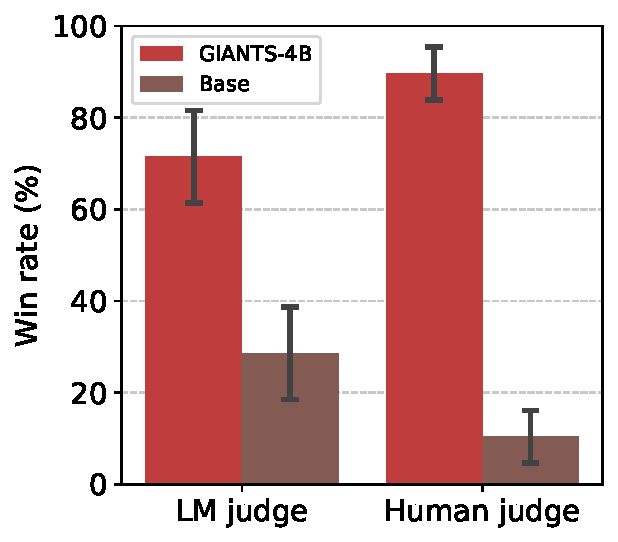
\includegraphics[width=0.9\linewidth]{figs/win_rate_human_eval_similarity.pdf}
    \vspace{-3mm}
    \caption{\footnotesize \textbf{Win rates for \ourmethod{}} \ourmethod{} achieves a higher win rate for similarity than the base model for both the LM and Human judge.} 
    \vspace{-3mm}
    \label{fig:win_rate_human_eval_similarity}
\end{wrapfigure}
\textbf{1) Insights generation is a challenging task even for large proprietary models.} Despite their success across diverse NLP benchmarks, current frontier models exhibit significant limitations in native idea synthesis. For instance, \qwenfourb{} achieves an average similarity score of only $4.75$ (Figure~\ref{fig:all_domain_radar_comparison_gemini-3-pro-preview_vs_Qwen3-14B}). Based on our LLM-based evaluation rubric (Figure~\ref{fig:similarity_judge_prompt}), a score in this range indicates that while generated insights may align topically with the ground truth, they fail to capture the core scientific contribution or technical nuance. Notably, significantly larger proprietary models, such as \gemtwopro{} and \gemthreepro{}, perform similarly to the smaller \qwenfourb{} baseline. This finding suggests that scientific ideation capabilities do not scale linearly with model size alone, reinforcing the necessity for specialized training paradigms like \ourmethod{}.

\begin{wrapfigure}{r}{0.4\textwidth}
    \centering
    \vspace{-2mm}
    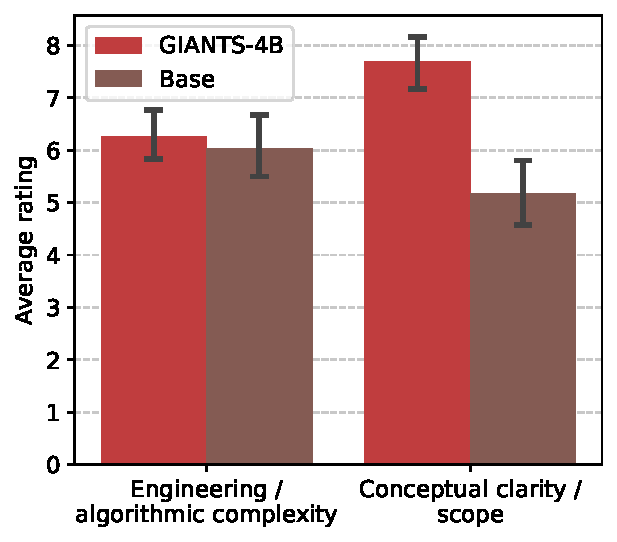
\includegraphics[width=0.9\linewidth]{figs/feasibility_bar_plot.pdf}
    \vspace{-3mm}
    \caption{\footnotesize \textbf{Feasibility Human Eval} Humans gauge the feasibility of a generated insight in 2 axes: (1) engineering/algorithmic complexity \& (2) conceptual clarity/scope, finding \ourmethod{} generates insights with similar algorithmic complexity and better clarity.} 
    \vspace{-3mm}
    \label{fig:feasibility_bar_plot}
\end{wrapfigure}
\textbf{2) Directly optimizing similarity scores significantly improves insight generation}
Our primary finding is that \ourmethod{} achieves the highest performance among all tested methods. By directly optimizing for similarity scores via reinforcement learning (RL), \ourmethod{} yields a relative improvement of 28\% on the full test set (Figure~\ref{fig:all_domain_radar_comparison_gemini-3-pro-preview_vs_Qwen3-14B}) and 34\% on the subset containing only unseen parent papers (Figure~\ref{fig:all_domain_radar_comparison_gemini-3-pro-preview_vs_Qwen3-14B_unseen_parents}) over \gemthreepro{}. In contrast, standard supervised fine-tuning (SFT) on ground-truth insights actually degrades performance, while the SFT-think variant only achieves parity with the base model. These results suggest that standard imitation learning is largely ineffective for this synthesis task; however, our RL framework successfully aligns the model's capabilities with high-quality human insights. This performance trend remains robust as we increase the number of samples to optimize the similarity score via inference-time scaling, as illustrated in Figure~\ref{fig:best_at_k}.

To further validate these gains, we employed the judge framework from \citet{tong2026ai} as an independent third-party evaluation of paper quality. In this setup, the judge model is fine-tuned to predict which of two papers is more likely to receive higher citations. We found that optimizing our similarity-based metric allows \ourmethod{} to achieve a 62\% win rate over the base model across $n=500$ insights across CS disciplines (Figure~\ref{fig:winrate_taste}). This evaluation accounts for potential biases, as in our similarity scoring, by ensuring order invariance and by filtering out inconsistent judgments.

\begin{figure}[t]
    \centering
    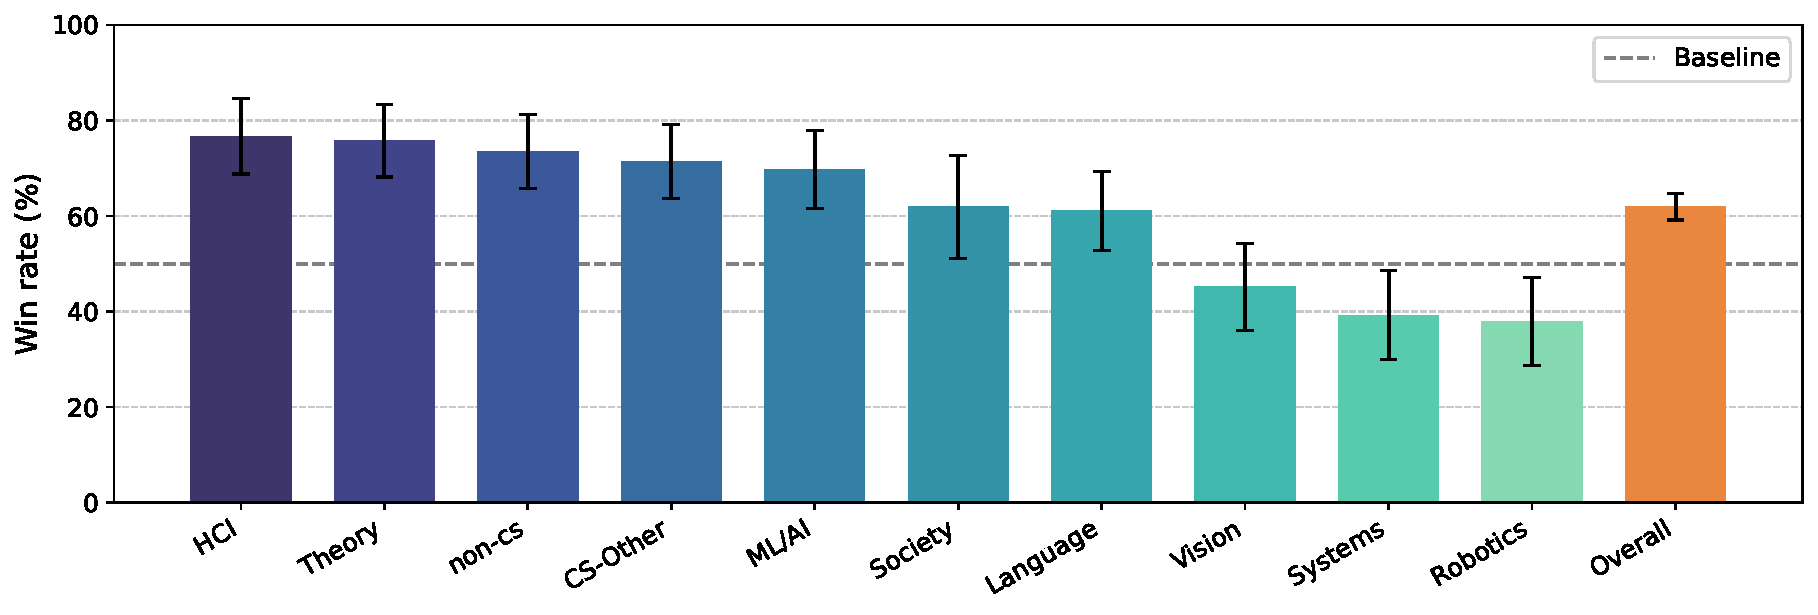
\includegraphics[width=0.9\linewidth]{figs/win_rate_taste_by_domain.pdf}
    \vspace{-3mm}
    \caption{\footnotesize \textbf{\ourmethod{} achieves a 62\% overall win rate against the Base model using SciJudge-30B.} We evaluate \ourmethod{} utilizing the judge framework from \citet{tong2026ai}, originally optimized for citation count prediction. While performance varies by domain, reaching up to a 76\% win rate in HCI but dropping to 37\% in robotics, \ourmethod{} maintains a robust overall win rate of 62\%.}
    \label{fig:winrate_taste}
    \vspace{-3mm}
\end{figure}
We supplemented this automated evaluation with two independent preliminary human studies to assess the real-world impact of our method. First, we measured the win rate of \ourmethod{} against the base model specifically regarding alignment with the downstream paper's actual insights (Figure~\ref{fig:win_rate_human_eval_similarity}). In this head-to-head comparison, \ourmethod{} achieved a $71.4\%$ win rate according to an LM judge and a $89.7\%$ win rate according to human evaluators. Finally, we assessed the feasibility of the generated insights across two axes: algorithmic complexity and conceptual clarity. Our analysis indicates that while \ourmethod{} produces insights of similar algorithmic complexity to the base model, it significantly improves conceptual clarity, making the generated ideas more interpretable and actionable. Further details regarding the human study methodology are provided in Appendix~\ref{app:human_eval}.

\begin{wrapfigure}{r}{0.4\textwidth}
    \centering
    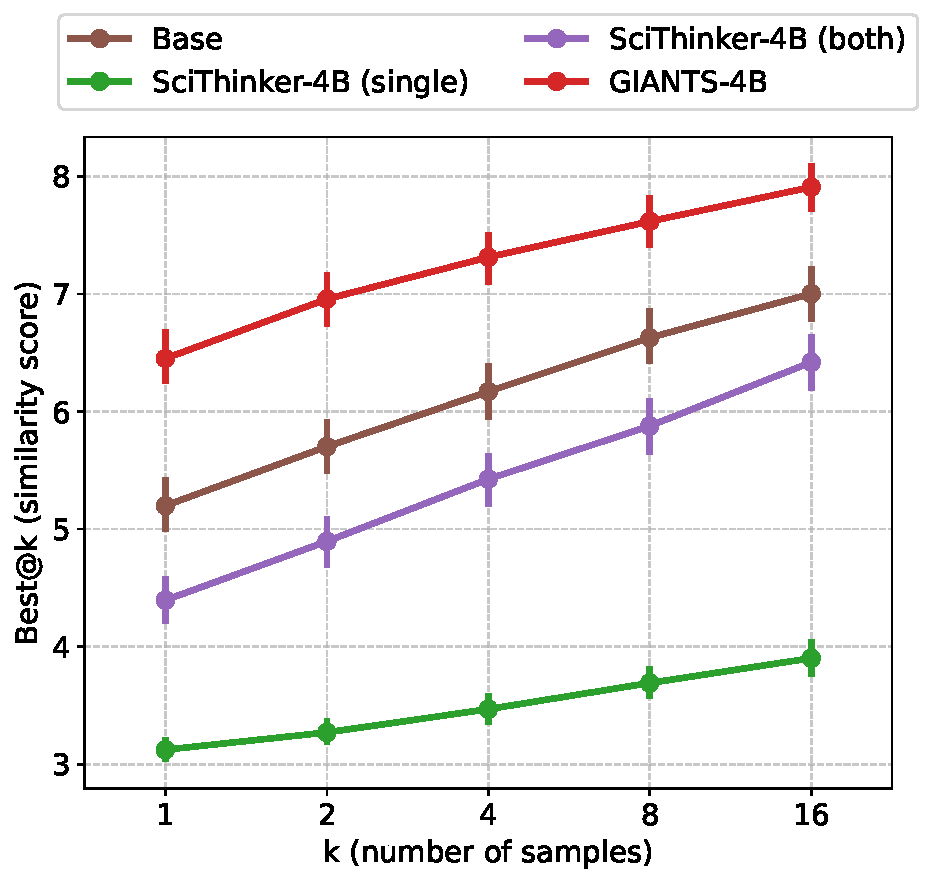
\includegraphics[width=\linewidth]{figs/best_at_k.pdf}
    \vspace{-3mm}
    \caption{\footnotesize \textbf{Test Time Inference of \ourmethod{}}. \ourmethod{} consistently outperforms the base model and other insight proposer methods such as SciThinker-4B~\citep{tong2026ai}, which is optimized for citation count (provided a single or both parent papers).}
    \vspace{-5mm}
    \label{fig:best_at_k}
\end{wrapfigure}
\textbf{3) \ourmethod{} zero-shot generalizes to new domains and distribution of parent papers}. 
Crucially, the synthesis capabilities acquired by \ourmethod{} are not restricted to its training data. Although trained exclusively on papers from the Language domain (CS.CL), we observed consistent performance gains across all evaluated disciplines as seen in Figure~\ref{fig:all_domain_radar_comparison_gemini-3-pro-preview_vs_Qwen3-14B}, including Physics, Quantitative Biology, and Economics. This suggests that the model learns a generalizable mechanism for combining disparate ideas rather than memorizing domain-specific heuristics. Furthermore, Figure~\ref{fig:all_domain_radar_comparison_gemini-3-pro-preview_vs_Qwen3-14B} and \ref{fig:all_domain_radar_comparison_gemini-3-pro-preview_vs_Qwen3-14B_unseen_parents} show the generalization on fully held out papers that appear temporally after the distribution of papers in the training set. 

% Has a lot of whitespace
% \begin{figure}[t]
%     \centering
%     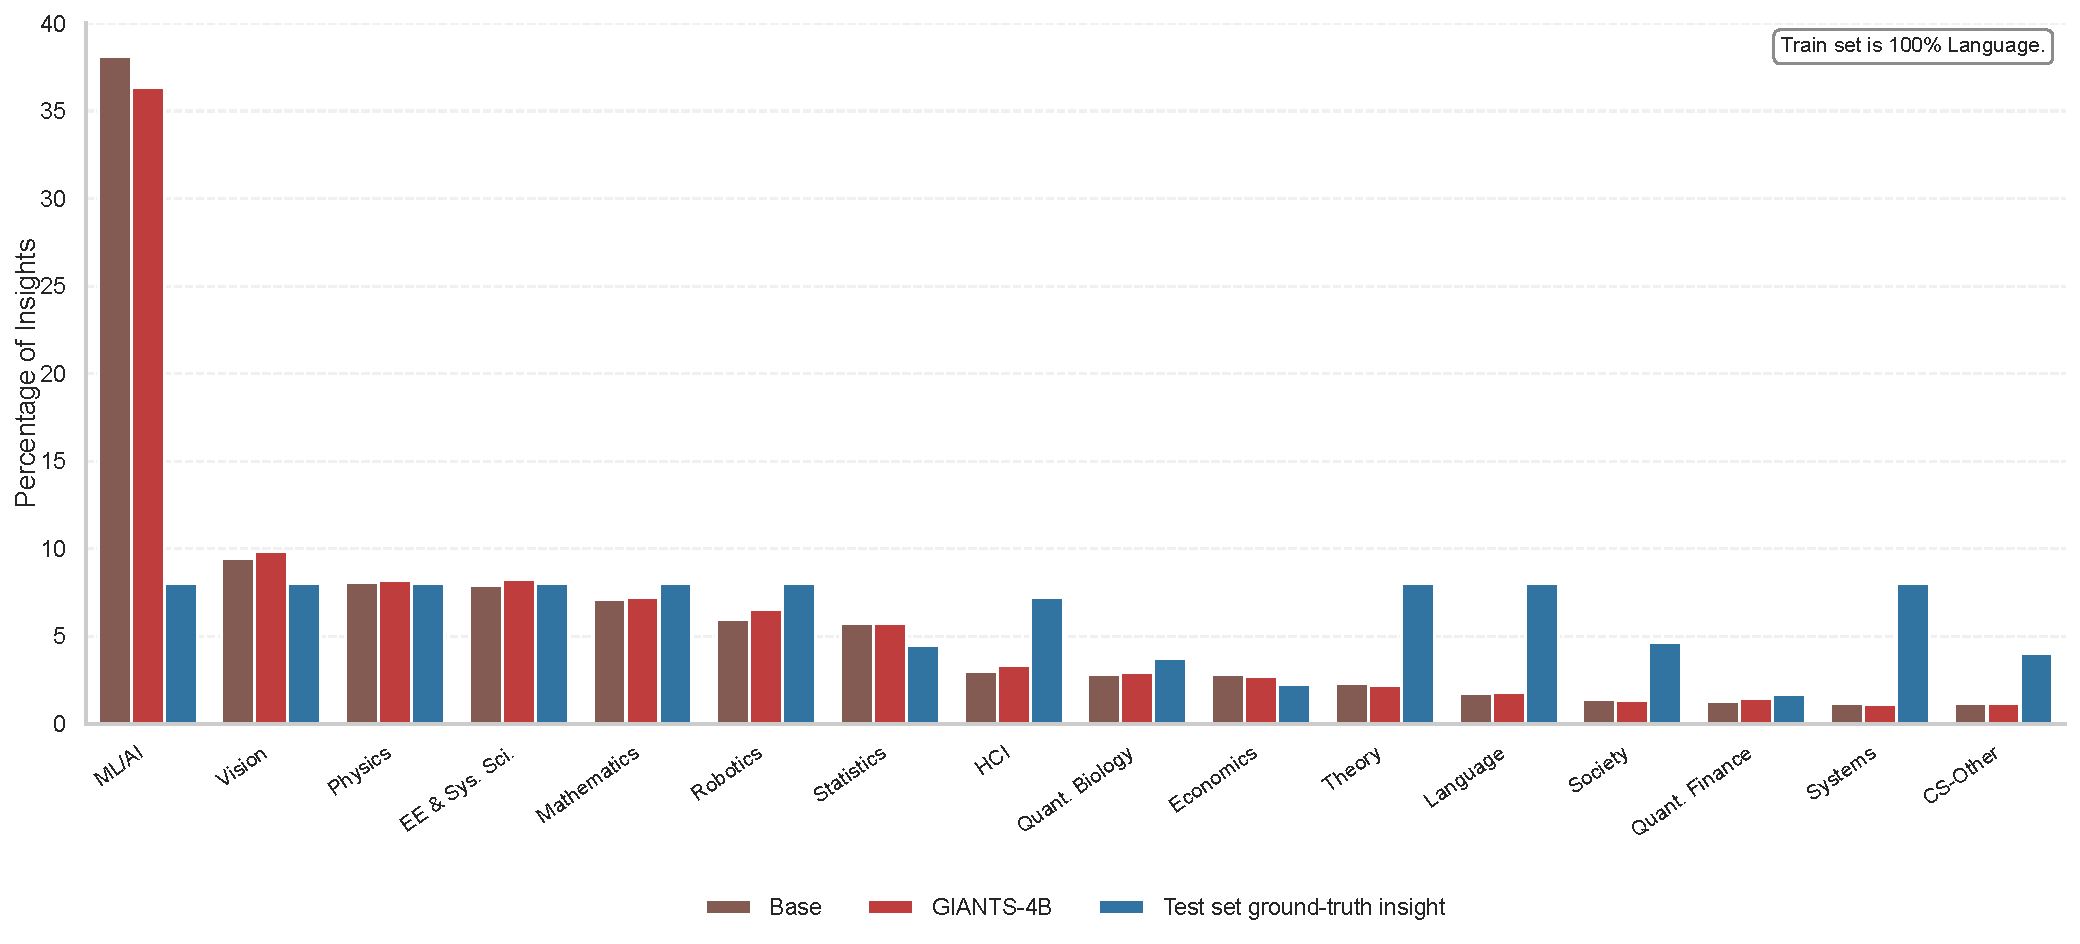
\includegraphics[width=0.9\linewidth]{figs/arxiv_distribution_plot_colorfix.pdf}
%     \vspace{-3mm}
%     \caption{\footnotesize \textbf{The diversity of insights generated by the base and RL models characterized by Gemini 3.1 Flash Lite.} RL fine-tuning for \ourmethod{} keeps a similar distribution of papers to the base model, despite being optimized solely on one domain (cs.CL).}
%     \vspace{-3mm}
%     \label{fig:arxiv_dist}
% \end{figure}

\textbf{Evaluation reliability check}. 
To ensure our findings are robust and that similarity scores are not biased toward the specific judge model that was used during training, we conducted a cross-model validation using an independent judge, \qwenfourteenb{} (Figure~\ref{fig:all_domain_radar_comparison_gemini-3-pro-preview_vs_Qwen3-14B}, right). This secondary evaluation corroborated our primary findings, ranking \ourmethod{} as the top-performing model across all metrics, albeit with a slightly more compressed performance margin. We also report results under three additional judge models in Appendix~\ref{appendix:ablations_with_diverse_lm_judges}, with consistent findings across model sizes.


% \begin{table}[t]
% \begin{center}
% \begin{tabular}{ll}
% \toprule
% \multicolumn{1}{c}{\bf Model}  &\multicolumn{1}{c}{\bf Similarity score on test} \\
% \midrule
% Base (\qwenfourb)         &$6.6$ \\
% RL (\qwenfourb)             &$7.64$ \\
% SFT (\qwenfourb)
% &$6.456$ \\

% SFT-think (\qwenfourb)
% &$6.674$ \\
% \gemtwopro            &$6.903$ \\   
% \gemthreepro             &$6.866$ \\ 
% \bottomrule
% \end{tabular}
% \end{center}\caption{RL outperforms the base model and other frontier models}\label{sample-table}
% \end{table}



% \begin{table}[t]
% \begin{center}
% \begin{tabular}{lcc}
% \toprule
% \multicolumn{1}{c}{\bf Model} 
% & \multicolumn{1}{c}{\bf Similarity score on test (judged by \qwenfourteenb{})} 
% & \multicolumn{1}{c}{\bf Similarity on test-unseen-parents ($N=341$)} \\
% \midrule
% Base (\qwenfourb)        & $7.174$   & $0$ \\
% % SFT (\qwenfourb)         & $6.456$ & $6.468$ \\
% % SFT-think (\qwenfourb)   & $6.674$ & $6.744$ \\
% % \gemtwopro{}               & $6.903$ & $7.038$ \\   
% \gemthreepro{}             & $7.229$ & $0$ \\ 
% RL (\qwenfourb)          & $\textbf{7.594}$  & $0$ \\
% \midrule
% \textit{Relative gain vs.\ Base (RL)} 
% & $\mathbf{+5.9\%}$ 
% & $\mathbf{0}$ \\
% \bottomrule
% \end{tabular}
% \end{center}
% \caption{RL outperforms the base model and other frontier models}
% \label{sample-table}
% \end{table}

% \begin{table}[t]
% \begin{center}
% \begin{tabular}{lcc}
% \toprule
% \multicolumn{1}{c}{\bf Model} 
% & \multicolumn{1}{c}{\bf Similarity score on test (judged by \gemtwopro{})} 
% & \multicolumn{1}{c}{\bf Similarity on test-unseen-parents ($N=341$)} \\
% \midrule
% Base (\qwenfourb)        & $6.526$   & $0$ \\
% % SFT (\qwenfourb)         & $6.456$ & $6.468$ \\
% % SFT-think (\qwenfourb)   & $6.674$ & $6.744$ \\
% % \gemtwopro{}               & $6.903$ & $7.038$ \\   
% \gemthreepro{}             & $6.948$ & $0$ \\ 
% RL (\qwenfourb)          & $\textbf{8.061}$  & $0$ \\
% \midrule
% \textit{Relative gain vs.\ Base (RL)} 
% & $\mathbf{+5.9\%}$ 
% & $\mathbf{0}$ \\
% \bottomrule
% \end{tabular}
% \end{center}
% \caption{RL outperforms the base model and other frontier models}
% \label{sample-table}
% \end{table}

% \begin{figure}[t]
% \begin{center}
% %\framebox[4.0in]{$\;$}
% \fbox{\rule[-.5cm]{0cm}{4cm} \rule[-.5cm]{4cm}{0cm}}
% \end{center}
% \caption{Sample figure caption.}
% \end{figure}
\begin{figure}[t]
    \centering
    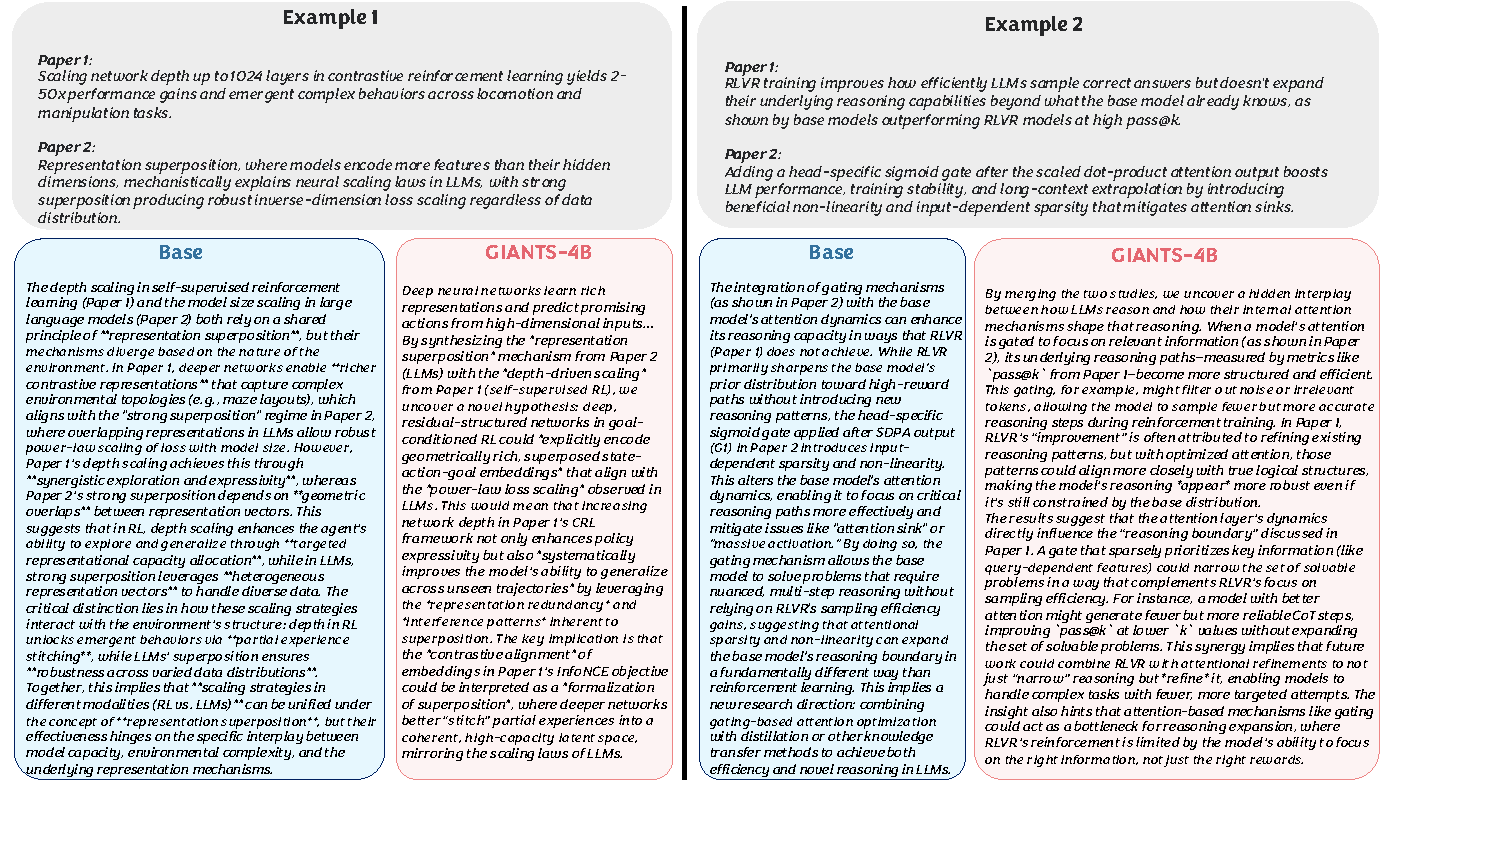
\includegraphics[width=\linewidth]{figs/qualitative.pdf}
    % 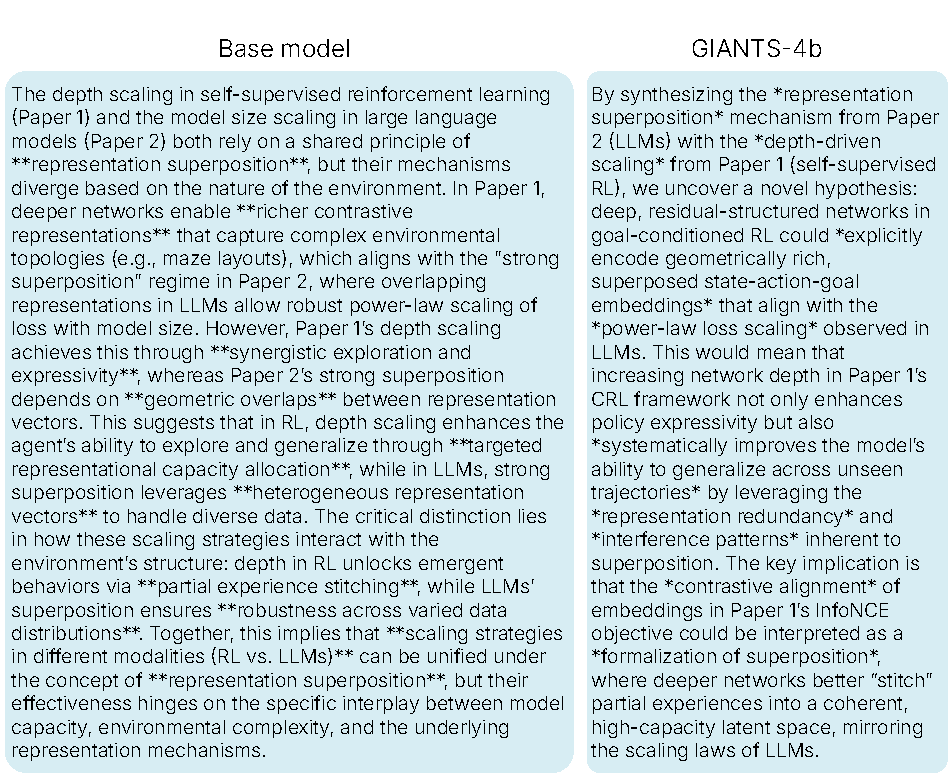
\includegraphics[width=0.43\linewidth]{figs/qualitative_1.pdf}
    % \hspace{3mm} \vrule \hspace{3mm}
    % 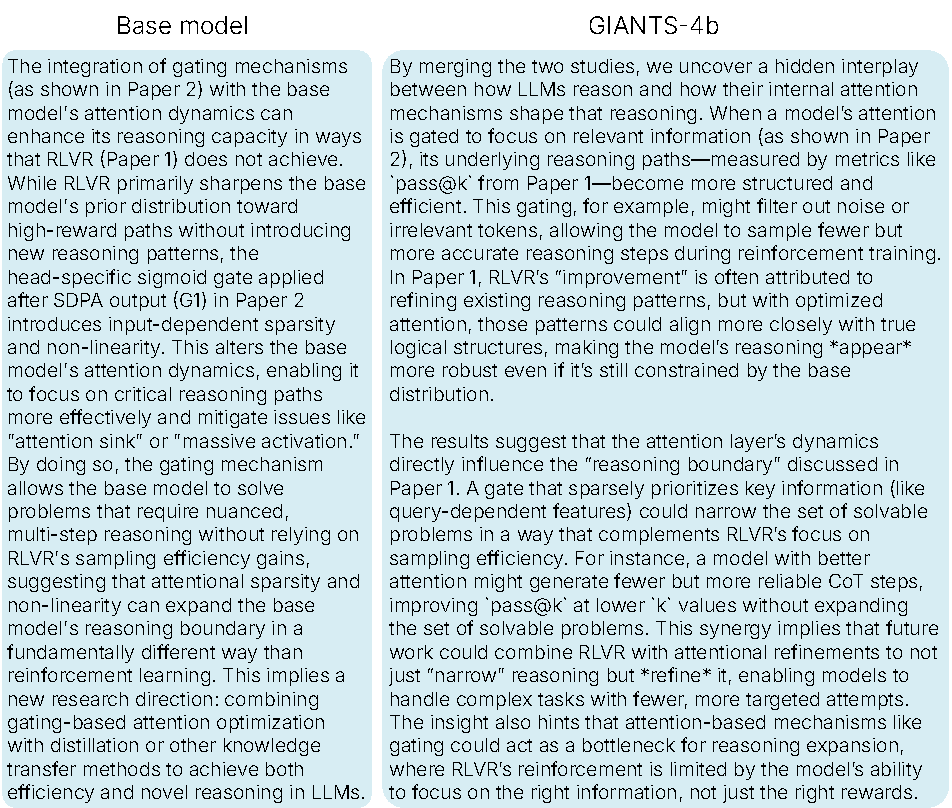
\includegraphics[width=0.4\linewidth]{figs/qualitative_2.pdf}
    \vspace{-3mm}
    \caption{\footnotesize \textbf{Qualitative comparison of insights derived from NeurIPS 2025 award-winning papers.} (Left) \ourmethod{} identifies a more concrete cross-paper mechanism than the base model (\qwenfourb{}). (Right) \ourmethod{} produces a grounded, meaningful contribution, avoiding the overly ambitious and infeasible propositions generated by the base model.}
    \label{fig:qualitative}
    \vspace{-3mm}
\end{figure}
\textbf{Qualitative Comparison of Models}
We present qualitative examples to demonstrate that our generated insights meaningfully integrate concepts from prior literature. To study this, we use NeurIPS 2025 award-winning papers as representative high-quality source material and compare the insights produced by \ourmethod{} against those generated by \qwenfourb{}.

First, Figure~\ref{fig:qualitative} (left) highlights an insight derived from two prior works \citep{wang20251000, liu2025superposition}. While the base model merely summarizes the parent papers without synthesizing a novel perspective, \ourmethod{} proposes a concrete mechanistic connection between the two studies that goes beyond the parent papers. Next, Figure~\ref{fig:qualitative}  (right) examines an insight based on two different papers \citep{yue2025does, qiu2025gated}. Here, the base model generates an overly ambitious claim, suggesting that gating mechanisms expand reasoning boundaries in ways that RLVR cannot, which is unsupported by the source texts. In contrast, \ourmethod{} remains grounded in the actual findings while still identifying a non-trivial connection: that attention gating may dictate how effectively reinforcement learning concentrates probability mass across useful reasoning trajectories. This comparison underscores a critical distinction between boldness and genuine insightfulness. Whereas the base model's novelty relies on unsupported extrapolation, \ourmethod{} maintains a narrower scope to identify a highly plausible interaction between the foundational works.

Overall, these two examples showcase the qualitative differences between the base model and \ourmethod{}, underscoring the properties of diversity and feasibility that are present in the insights that are generated.

\begin{AIbox}{Takeaways of Experimental Evaluation}
\ourmethod{} significantly outperforms both frontier models and supervised fine-tuning at generating feasible, high-quality scientific insights. Furthermore, despite training exclusively on a single domain, the model successfully zero-shot generalizes its synthesis capabilities across diverse, unseen scientific disciplines and temporally held-out literature.
\end{AIbox}




